
%opening
\title{Animation der TableView}
\author{Burak Erol, Philipp Winterholler}

\section{Animation der TableView}

Um eine Übersicht aller gefundenen \SEARCH-Tags grafisch darzustellen, wurde ein Label über den \SECH-Button ergänzt, welche die Anzahl der \SEARCH-Tags in einer roten Schrift angibt. Diese Anzahl soll dem Nutzer zeigen, wie viele \SEARCH-Tags sich auf der Webseite befinden. Beim Bedienen des \SECH-Buttons, wird die \SEARCH-Tabelle animiert herbei gerufen. Diese Tabelle wird rechts im Browser ein- und ausgefahren. Das WKWebView wird dementsprechend vergrößert oder verkleinert. Bedient man diesen \SECH-Button, so fährt sich eine Tabelle vom rechten Bildschirm aus und liefert alle Tags in einer TableView zurück. Die zurückgelieferten Tags werden in seperaten Zellen auf der TableView abgespeichert, die durch anklicken eine neue Pop-Up Seite, spezifisch zu dem angeklickten Tag, öffnet. Aufgrund der Umstellung der Navigationsleiste wird diese grafische Darstellung der Anzahl an \SECH-Tags nicht mehr angezeigt. Die Umstellung der Navigationsleiste war notwendig um die Höhe und Breite des WKWebViews festzulegen, darum ist ein neuer Navigation Controller erzeugt worden, welche die Navigation Bar automatisch mitliefert. In die neue Navigation Bar kann jedoch kein Label hinzugefügt und spezifisch positioniert werden, somit wurde diese Option entfernt.

\begin{figure}
	\centering
	
\includegraphics[width=12cm]{Sech_Anzahl}
	\caption{Anzahl der \SEARCH-Tags}
	\label{fig:Anzahl}
\end{figure}

\pagebreak

\begin{figure}
	\centering
	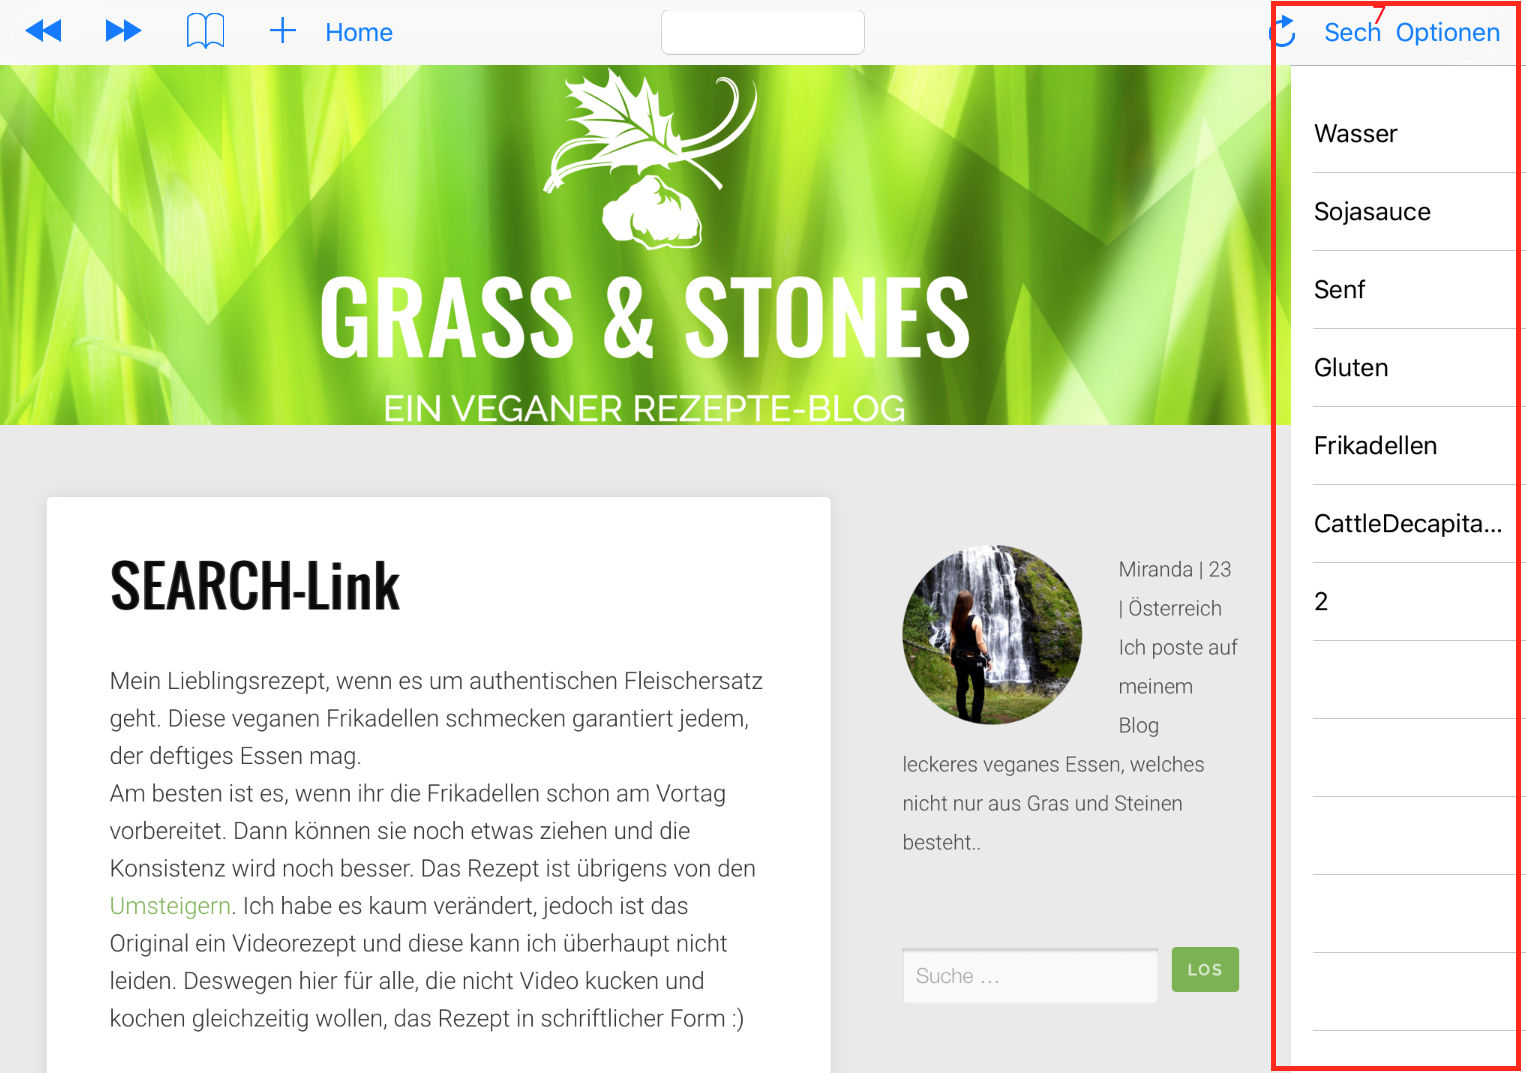
\includegraphics[width=12cm]{Sech_Tabelle_aufgeklappt}
	\caption{\SEARCH-Tabelle aufgeklappt}
	\label{fig:aufgeklappt}
\end{figure}

\pagebreak

\begin{figure}
	\centering
	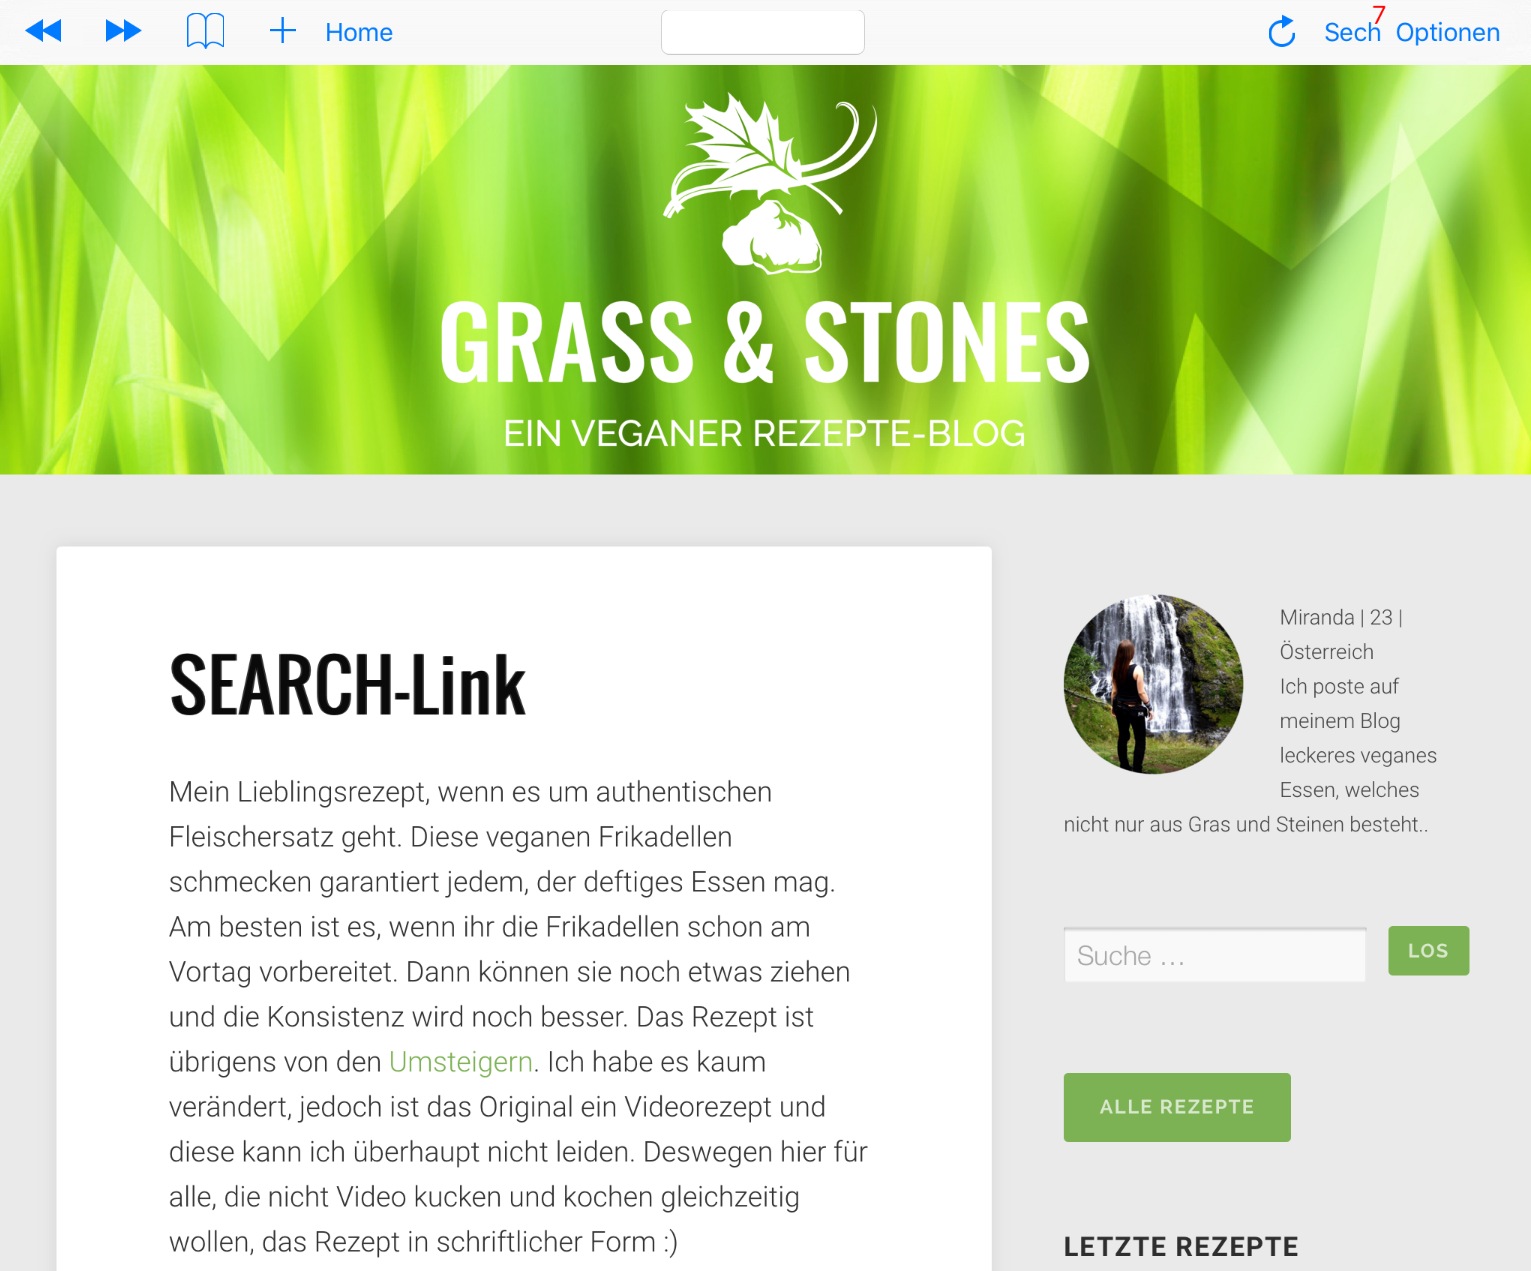
\includegraphics[width=12cm]{Sech_Tabelle_versteckt}
	\caption{\SEARCH-Tabelle versteckt}
	\label{fig:}
\end{figure}
